
% ════════════════════════════════════════════
% 模型准备（5.2.2.模型准备.tex，三级子块）
% ════════════════════════════════════════════
\subsubsection{模型准备}

\textbf{1.数据预处理}

附件二提供了 2025 年全年 365 天、每天 144 个 10 分钟时间点的小区负载与光伏实际功率数据，数据量约为 $365\times 144$ 的两张二维矩阵。为便于逐日建模，需要对数据进行时间对齐、数值化与按天切分。设第 $d$ 天第 $k$ 个间隔的负载与光伏功率分别为 $L_{d,k}$ 与 $S_{d,k}$，则全年数据可组织为：
\begin{equation}
    \boldsymbol{L}=[L_{d,k}]_{365\times 144},\quad \boldsymbol{S}=[S_{d,k}]_{365\times 144}
\end{equation}
其中，$d=0,1,\dots,364$ 表示天数序号，$k$ 表示日内间隔序号。对两张矩阵逐元素执行数值化检查，全年缺失值为零，负载分布于 $1995.7\sim 7978.9$ kW，光伏分布于 $0\sim 10216.2$ kW。预处理前后对比如图\ref{fig:preprocess2}所示。

\begin{figure}[H]
    \centering
    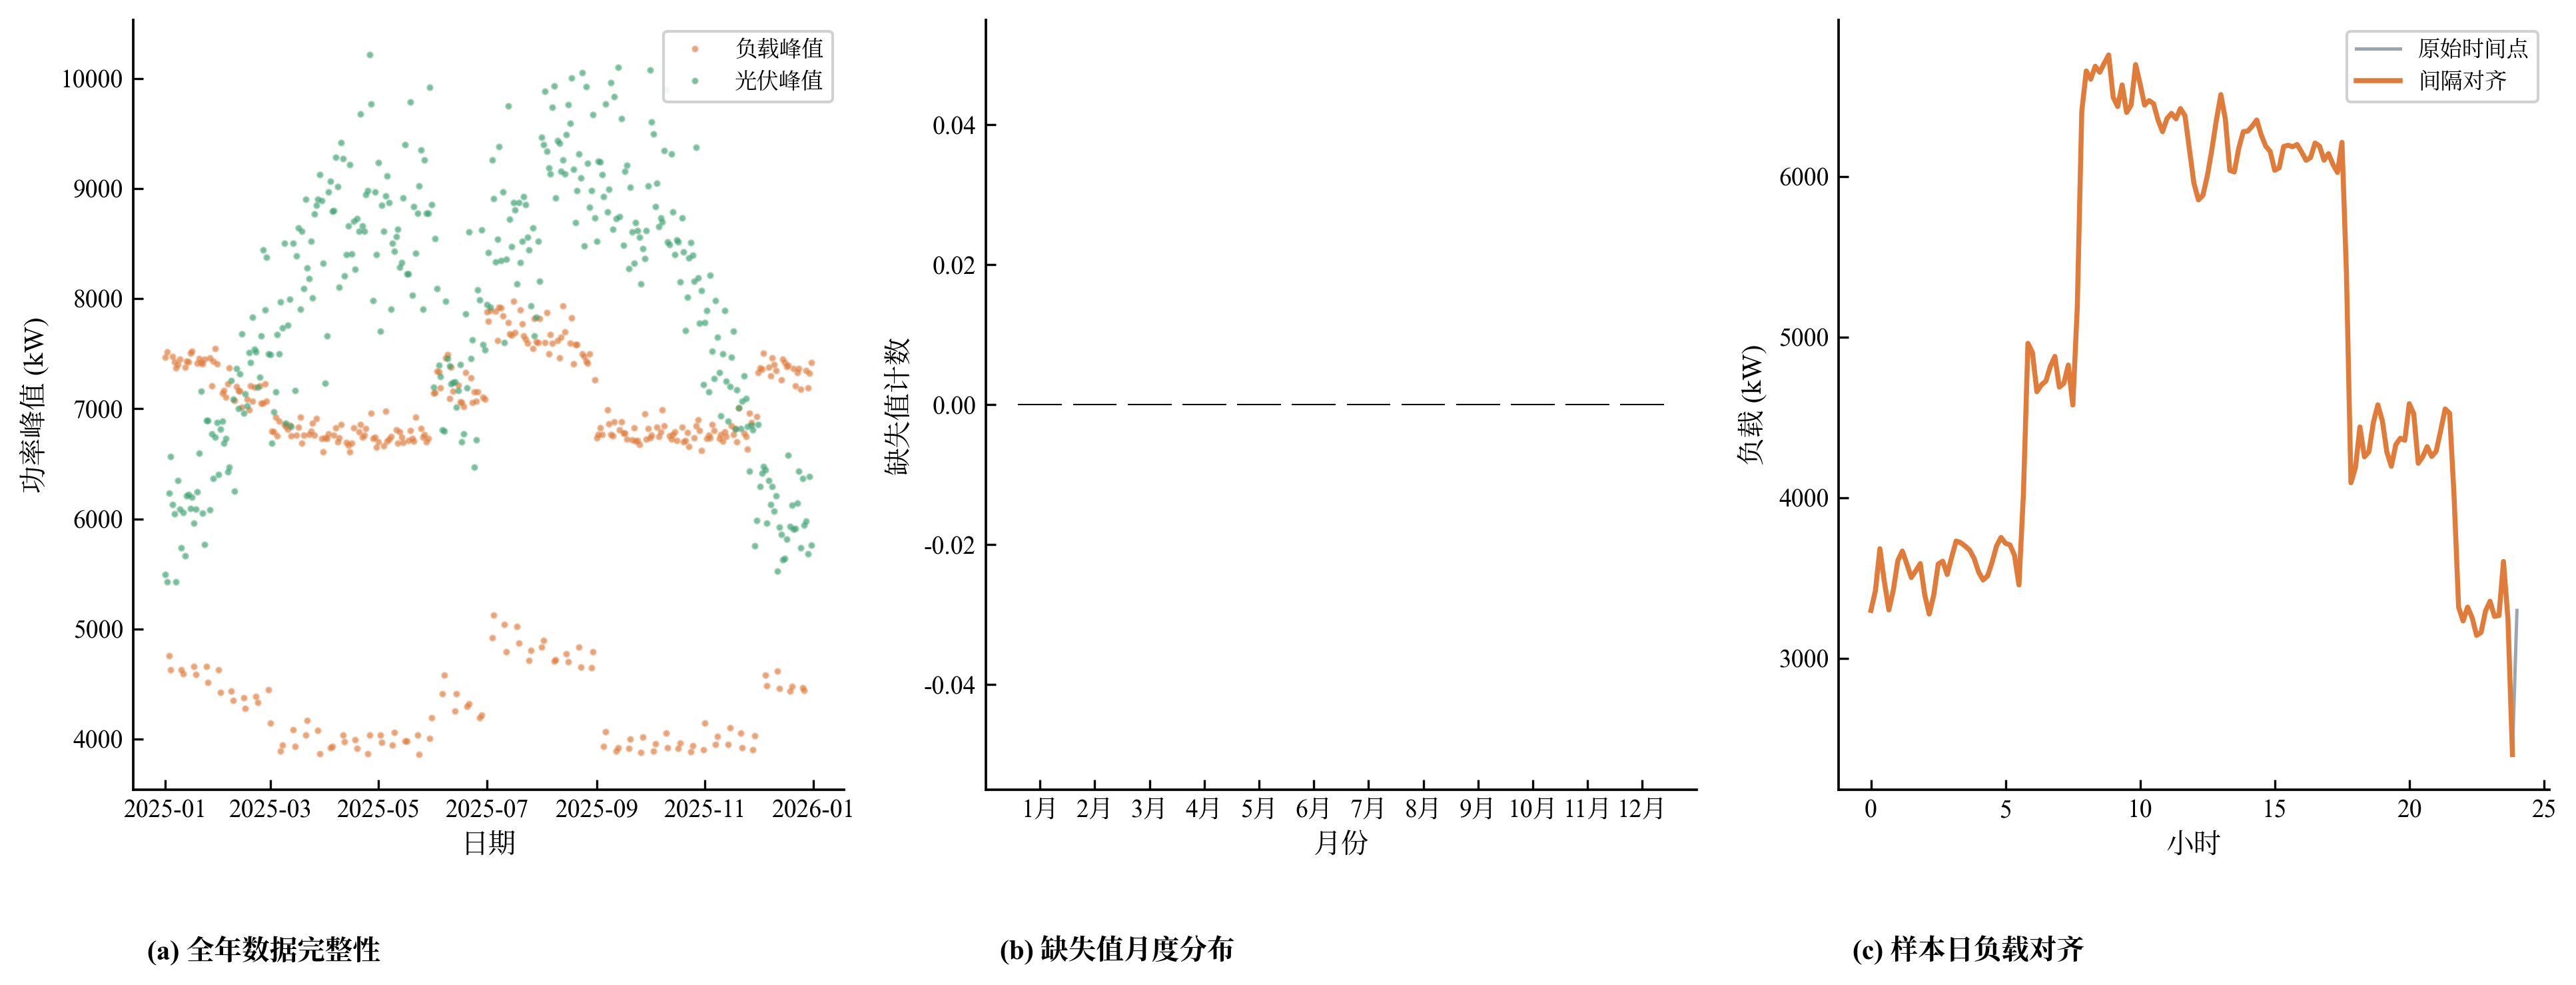
\includegraphics[width=0.72\textwidth]{../求解/问题二/图片/图2-1_预处理前后对比.png}
    \caption{问题二全年数据预处理与完整性检查}
    \label{fig:preprocess2}
\end{figure}

由图\ref{fig:preprocess2}可知，全年负载与光伏峰值逐日变化，负载呈现明显的季节波动而光伏呈现冬低夏高的规律，且全年无缺失数据，样本日负载曲线在时间对齐后与原始时间点序列完全一致，数据质量良好。

需要说明的是，附件 2 的 365 天数据中，2025 年 1 月（1 月 1 日—1 月 31 日）作为\textbf{预热期}：模型以 1 月 1 日 0:00 储电量 6000 kWh 为初值逐日滚动，使储电量摆脱初始条件影响、进入稳定日循环（2 月 1 日 0:00 储电量已收敛至 1200 kWh 下限）；按照附件 5 的要求，结果文件与后文所有费用汇总均只统计 2025 年 2 月 1 日至 12 月 31 日共 334 天。

\textbf{2.算法选择}

在完成数据预处理后，本问需在全年尺度上求解 365 个逐日优化问题。与问题一相同，每个子问题均为线性规划，可直接沿用线性规划算法；区别在于需要设计日间储电量的传递机制。可从建模复杂度与全局最优性两个维度比较独立逐日求解与全年统一求解两种策略，如表\ref{tab:algo2}所示。

\begin{longtable}{>{\centering\arraybackslash}p{0.22\textwidth}>{\centering\arraybackslash}p{0.24\textwidth}>{\centering\arraybackslash}p{0.22\textwidth}>{\centering\arraybackslash}p{0.20\textwidth}}
  \caption{问题二求解策略对比}
  \label{tab:algo2} \\
  \toprule
  策略 & 建模复杂度 & 计算规模 & 最优性 \\
  \midrule
  \endfirsthead
  \caption{问题二求解策略对比（续）} \\
  \toprule
  策略 & 建模复杂度 & 计算规模 & 最优性 \\
  \midrule
  \endhead
  \bottomrule
  \endfoot
  全年统一求解 & 高 & 大规模 & 严格全局最优 \\
  逐日滚动求解 & 低 & 小规模 & 近似最优 \\
\end{longtable}

如\ref{tab:algo2}所示，全年统一求解虽在数学上严格，但变量规模达数十万，求解开销大；由于本问每日电价完全相同，日间不存在跨日套利空间，逐日滚动求解在储电量仅受上下限约束、无日末固定值的条件下，与全年统一求解的结果高度一致，且计算量小、易于解释。综合以上分析，本问选择逐日滚动线性规划策略进行求解。
